%%%%%%%%%%%%%%%%%%%%%%%%%%%%%%%%%%%%%%%
\documentclass{article}
\usepackage{graphicx}
\documentclass{article}
\usepackage[demo]{graphicx}
\usepackage{caption}
\usepackage{subcaption}

%%%%%%%%%%%%%%%%%%%%%%%%%%%%%%%%%%%%%%%%%
% Lachaise Assignment
% Structure Specification File
% Version 1.0 (26/6/2018)
%
% This template originates from:
% http://www.LaTeXTemplates.com
%
% Authors:
% Marion Lachaise & François Févotte
% Vel (vel@LaTeXTemplates.com)
%
% License:
% CC BY-NC-SA 3.0 (http://creativecommons.org/licenses/by-nc-sa/3.0/)
% 
%%%%%%%%%%%%%%%%%%%%%%%%%%%%%%%%%%%%%%%%%

%----------------------------------------------------------------------------------------
%	PACKAGES AND OTHER DOCUMENT CONFIGURATIONS
%----------------------------------------------------------------------------------------

\usepackage{amsmath,amsfonts,stmaryrd,amssymb} % Math packages

\usepackage{enumerate} % Custom item numbers for enumerations

\usepackage[ruled]{algorithm2e} % Algorithms

\usepackage[framemethod=tikz]{mdframed} % Allows defining custom boxed/framed environments

\usepackage{listings} % File listings, with syntax highlighting
\lstset{
	basicstyle=\ttfamily, % Typeset listings in monospace font
}

%----------------------------------------------------------------------------------------
%	DOCUMENT MARGINS
%----------------------------------------------------------------------------------------

\usepackage{geometry} % Required for adjusting page dimensions and margins

\geometry{
	paper=a4paper, % Paper size, change to letterpaper for US letter size
	top=2.5cm, % Top margin
	bottom=3cm, % Bottom margin
	left=2.5cm, % Left margin
	right=2.5cm, % Right margin
	headheight=14pt, % Header height
	footskip=1.5cm, % Space from the bottom margin to the baseline of the footer
	headsep=1.2cm, % Space from the top margin to the baseline of the header
	%showframe, % Uncomment to show how the type block is set on the page
}

%----------------------------------------------------------------------------------------
%	FONTS
%----------------------------------------------------------------------------------------

\usepackage[utf8]{inputenc} % Required for inputting international characters
\usepackage[T1]{fontenc} % Output font encoding for international characters

\usepackage{XCharter} % Use the XCharter fonts

%----------------------------------------------------------------------------------------
%	COMMAND LINE ENVIRONMENT
%----------------------------------------------------------------------------------------

% Usage:
% \begin{commandline}
%	\begin{verbatim}
%		$ ls
%		
%		Applications	Desktop	...
%	\end{verbatim}
% \end{commandline}

\mdfdefinestyle{commandline}{
	leftmargin=10pt,
	rightmargin=10pt,
	innerleftmargin=15pt,
	middlelinecolor=black!50!white,
	middlelinewidth=2pt,
	frametitlerule=false,
	backgroundcolor=black!5!white,
	frametitle={Command Line},
	frametitlefont={\normalfont\sffamily\color{white}\hspace{-1em}},
	frametitlebackgroundcolor=black!50!white,
	nobreak,
}

% Define a custom environment for command-line snapshots
\newenvironment{commandline}{
	\medskip
	\begin{mdframed}[style=commandline]
}{
	\end{mdframed}
	\medskip
}

%----------------------------------------------------------------------------------------
%	FILE CONTENTS ENVIRONMENT
%----------------------------------------------------------------------------------------

% Usage:
% \begin{file}[optional filename, defaults to "File"]
%	File contents, for example, with a listings environment
% \end{file}

\mdfdefinestyle{file}{
	innertopmargin=1.6\baselineskip,
	innerbottommargin=0.8\baselineskip,
	topline=false, bottomline=false,
	leftline=false, rightline=false,
	leftmargin=2cm,
	rightmargin=2cm,
	singleextra={%
		\draw[fill=black!10!white](P)++(0,-1.2em)rectangle(P-|O);
		\node[anchor=north west]
		at(P-|O){\ttfamily\mdfilename};
		%
		\def\l{3em}
		\draw(O-|P)++(-\l,0)--++(\l,\l)--(P)--(P-|O)--(O)--cycle;
		\draw(O-|P)++(-\l,0)--++(0,\l)--++(\l,0);
	},
	nobreak,
}

% Define a custom environment for file contents
\newenvironment{file}[1][File]{ % Set the default filename to "File"
	\medskip
	\newcommand{\mdfilename}{#1}
	\begin{mdframed}[style=file]
}{
	\end{mdframed}
	\medskip
}

%----------------------------------------------------------------------------------------
%	NUMBERED QUESTIONS ENVIRONMENT
%----------------------------------------------------------------------------------------

% Usage:
% \begin{question}[optional title]
%	Question contents
% \end{question}

\mdfdefinestyle{question}{
	innertopmargin=1.2\baselineskip,
	innerbottommargin=0.8\baselineskip,
	roundcorner=5pt,
	nobreak,
	singleextra={%
		\draw(P-|O)node[xshift=1em,anchor=west,fill=white,draw,rounded corners=5pt]{%
		Question \theQuestion\questionTitle};
	},
}

\newcounter{Question} % Stores the current question number that gets iterated with each new question

% Define a custom environment for numbered questions
\newenvironment{question}[1][\unskip]{
	\bigskip
	\stepcounter{Question}
	\newcommand{\questionTitle}{~#1}
	\begin{mdframed}[style=question]
}{
	\end{mdframed}
	\medskip
}

%----------------------------------------------------------------------------------------
%	WARNING TEXT ENVIRONMENT
%----------------------------------------------------------------------------------------

% Usage:
% \begin{warn}[optional title, defaults to "Warning:"]
%	Contents
% \end{warn}

\mdfdefinestyle{warning}{
	topline=false, bottomline=false,
	leftline=false, rightline=false,
	nobreak,
	singleextra={%
		\draw(P-|O)++(-0.5em,0)node(tmp1){};
		\draw(P-|O)++(0.5em,0)node(tmp2){};
		\fill[black,rotate around={45:(P-|O)}](tmp1)rectangle(tmp2);
		\node at(P-|O){\color{white}\scriptsize\bf !};
		\draw[very thick](P-|O)++(0,-1em)--(O);%--(O-|P);
	}
}

% Define a custom environment for warning text
\newenvironment{warn}[1][Warning:]{ % Set the default warning to "Warning:"
	\medskip
	\begin{mdframed}[style=warning]
		\noindent{\textbf{#1}}
}{
	\end{mdframed}
}

%----------------------------------------------------------------------------------------
%	INFORMATION ENVIRONMENT
%----------------------------------------------------------------------------------------

% Usage:
% \begin{info}[optional title, defaults to "Info:"]
% 	contents
% 	\end{info}

\mdfdefinestyle{info}{%
	topline=false, bottomline=false,
	leftline=false, rightline=false,
	nobreak,
	singleextra={%
		\fill[black](P-|O)circle[radius=0.4em];
		\node at(P-|O){\color{white}\scriptsize\bf i};
		\draw[very thick](P-|O)++(0,-0.8em)--(O);%--(O-|P);
	}
}

% Define a custom environment for information
\newenvironment{info}[1][Info:]{ % Set the default title to "Info:"
	\medskip
	\begin{mdframed}[style=info]
		\noindent{\textbf{#1}}
}{
	\end{mdframed}
}
 % Include the file specifying the document structure and custom commands

%----------------------------------------------------------------------------------------
%	ASSIGNMENT INFORMATION
%----------------------------------------------------------------------------------------

\title{Project #1: Fast Trajectory Replanning} % Title of the assignment

\author{Vishnu Dhanasekaran, Swarnendu Roy, Nikhil Kulkarni \\ \texttt{netID: vd247, skr81, nsk62}} % Author name and email address

\date{Rutgers University --- July 13, 2020} % University, school and/or department name(s) and a date

%----------------------------------------------------------------------------------------

\begin{document}

\maketitle % Print the title



\section*{Part 0: Setup your Environments}
\subsubsection*{You will perform all your experiments in the same 50 grid-worlds of size
101 × 101. You first need to generate these environments appropriate.}
To generate our 50 101x101 grids we ran the provided gird-world-generator.py file and read and stored them into a 2D list. 

\section*{Part 1: Understanding the Methods} % Unnumbered section
\setcounter{fig}{0}

\begin{figure}[h!]
  
  \centering
  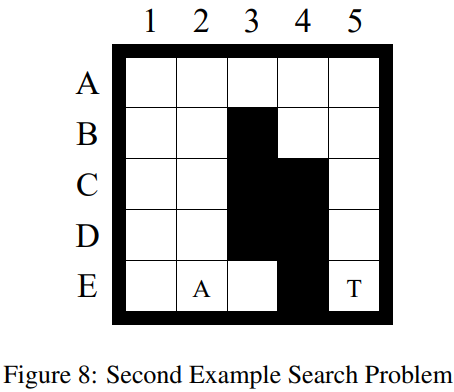
\includegraphics[width=0.5\textwidth]{east.png}
\end{figure}

\subsubsection*{Explaining why the agent chooses to go east rather than north}
The agent initially starts at cell E2, agent can now see all of the nodes that are neighboring the cell E2, these are (E3 f(3), E1 f(5), D2 f(5)) with g for all the nodes at 1. These nodes are added to the open list heap after their g(cost), h(heuristic) and f(g + h) values are updated. Once this is done, we pop the heap, which orders them in increasing order of f values, starting at E3. When the heap is popped the cell E3 will be popped before the other two and we will perform A* search on that E3. This is because according the heuristic E3 has a lower value while the cost of going to all the nodes stay the same, hence E3's f value is lower. Hence the agent will prefer to move east first.

\subsubsection*{This project argues that the agent is guaranteed to reach the target if it is not separated from it by blocked cells. Give a convincing argument that the agent in finite grid worlds indeed either reaches the target or discovers that this is impossible in finite time.}

If the grid space is a finite space then A* search can find a solution in finite time through exhaustively searching the grid, assuming that there is no blocked cells. Since every step's cost increases by one and every step also generates a finite number of neighbors, we will eventually be able to find a solution. One can argue that we may expand the same nodes more than once and get stuck in a loop, to avoid this we have implemented a closed list that stores the nodes that have already been expanded avoiding any repeats.


\section*{Part 2: The Effect of Ties}
\subsubsection*{Repeated Forward A* needs to break ties to decide which cell to expand next if
several cells have the same smallest f-value. It can either break ties in favor of cells with smaller g-values or in favor of
cells with larger g-values. Implement and compare both versions of Repeated Forward A* with respect to their run time or,
equivalently, number of expanded cells. Explain your observations in detail, that is, explain what you observed and give a
reason for the observation.}


\begin{figure}[h!]
  \centering
  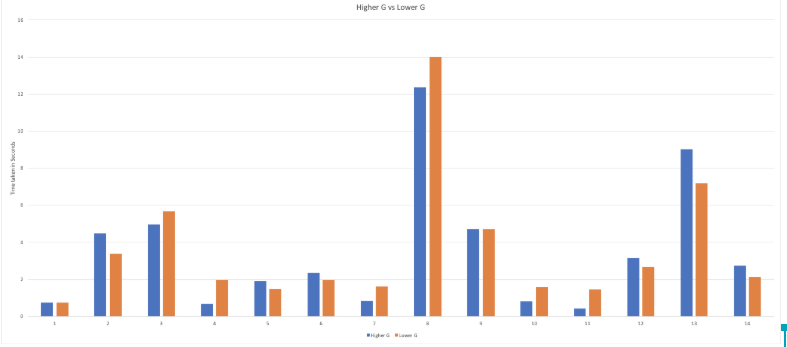
\includegraphics[width=0.8\textwidth]{graph1.png}
  \caption{Avg run-times: higher G: 3.51s, lower G: 4.62s
}
\end{figure}

After running our experiments over 50 different grids, ignoring the grids where a path was not found we see that, tie-breaking with a lower g(x) value results in a much higher run-time than a higher g(x). This is can be seen in the graph above.\\
This can be attributed to the fact the lower g(x) value results in considerably more expansions than using higher g(x) which is visualized by the two screenshots provided. This happens because the lower g(x) algorithm expands more nodes near the start. The cases where the lower g(x) has a better run-time can be attributed to more blocked nodes being present near the start.\\
Both search algorithms were run on the same 101x101 grid. Lower g(x) gives more than 1000 expansions which then causes a much higher run time. 

\\
\\
\textbf{After a run with greater g(x) value tie-breaking the results are as follows:}

\begin{figure}[h!]
\centerline{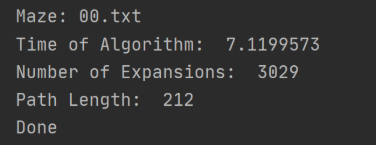
\includegraphics[scale=.5]{highergtie.png}}
\label{fig}
\end{figure}

\textbf{We can compare this to the lower g(x) value tie-breaking: }

\begin{figure}[h!]
\centerline{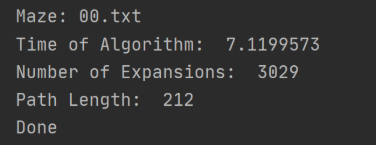
\includegraphics[scale=.5]{lowergtie.png}}
\label{fig}
\end{figure}

\clearpage

\section*{Part 3: Forward vs Backward}
\subsubsection*{Implement and compare Repeated Forward A* and Repeated Backward A*
with respect to their run-time or, equivalently, number of expanded cells. Explain your observations in detail, that is, explain
what you observed and give a reason for the observation. Both versions of Repeated A* should break ties among cells with
the same f-value in favor of cells with larger g-values and remaining ties in an identical way, for example randomly.}

\begin{figure}[h!]
  \centering
  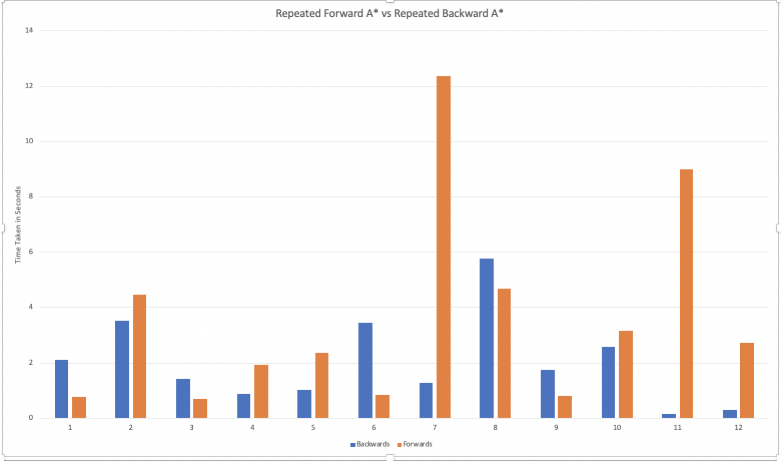
\includegraphics[width=0.8\textwidth]{graph2.png}
  \caption{Avg run-times: Repeated Forward A*: 3.51s, Repeated Backward A*: 2.29s

}
\end{figure}

On running Repeated Forwards A and Repeated Backwards A, we find that for some cases Repeated Forwards A is faster than Repeated Backwards A but for certain cases, Repeated Backwards A runs quicker than Repeated Forwards A and hence the run-time is varying but on an average it favors backwards. The favoring of backwards is due to the nature of the formed grid. This can be attributed to the fact that there may be potential bias in the positioning of the start and goal. It can be seen that if there are more blocked nodes around the position of wherever the agent’s starting position nodes, it leads to less expansion of nodes and a quicker run-time.

Given below we run both algorithms on two separate grids which gives us the different cases. We show pictures of the grids with the path, blocked and unblocked nodes, and also the run-times of the algorithms on each grid.

\\
The start is marked in green and the goal is marked in red.
We see near the start there are more blocked nodes than near the goal which causes the better run-time as shown below.
\newpage
\setcounter{figure}{0}
\textbf{Here is an example of grid favoring Forwards A*:}
\begin{figure}[h!]
\begin{subfigure}{.5\textwidth}
  \centering
  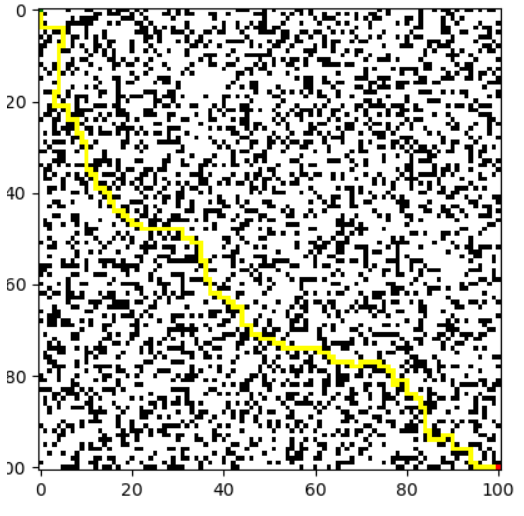
\includegraphics[width=.8\linewidth]{forwardA.png}
  \label{fig:sfig1}
\end{subfigure}%
\begin{subfigure}{.5\textwidth}
  \centering
  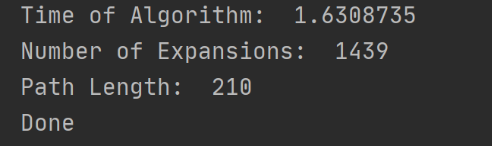
\includegraphics[width=.8\linewidth]{forwardAstats.png}
  \label{fig:sfig2}
\end{subfigure}
\caption{Faster Forward A*}
\label{fig:fig}
\end{figure}

\begin{figure}[h!]
\begin{subfigure}{.5\textwidth}
  \centering
  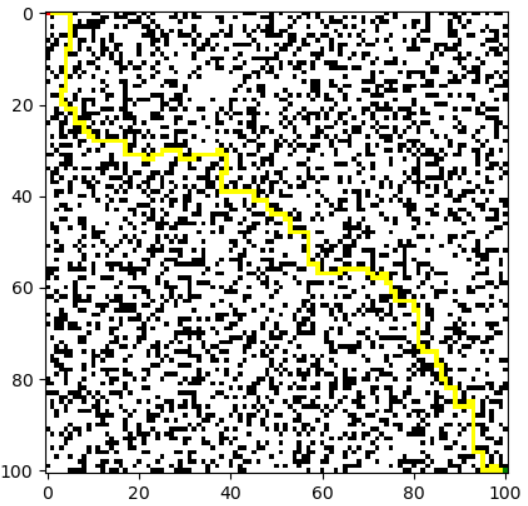
\includegraphics[width=.8\linewidth]{backwardsA.png}
  \label{fig:sfig1}
\end{subfigure}%
\begin{subfigure}{.5\textwidth}
  \centering
  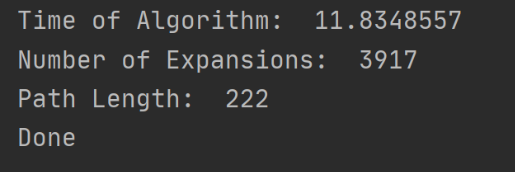
\includegraphics[width=.8\linewidth]{backwardsAstats.png}
  \label{fig:sfig2}
\end{subfigure}
\caption{Slower Backward A*}
\label{fig:fig}
\end{figure}

\textbf{Example of a grid favoring Backwards A*:}
\begin{figure}[h!]
\begin{subfigure}{.5\textwidth}
  \centering
  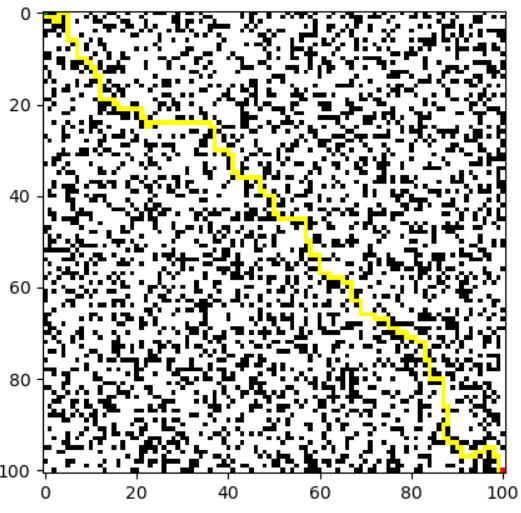
\includegraphics[width=.8\linewidth]{fastfrontA.png}
  \label{fig:sfig1}
\end{subfigure}%
\begin{subfigure}{.5\textwidth}
  \centering
  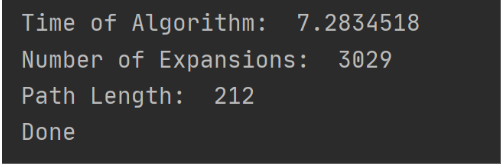
\includegraphics[width=.8\linewidth]{fastfrontAstats.png}
  \label{fig:sfig2}
\end{subfigure}
\caption{Slower Forward A*}
\label{fig:fig}
\end{figure}

\begin{figure}[h!]
\begin{subfigure}{.5\textwidth}
  \centering
  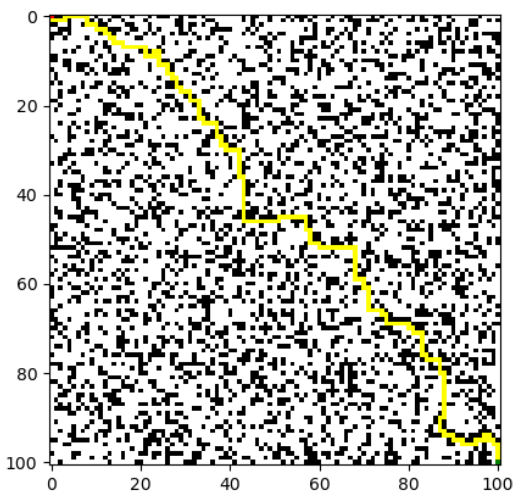
\includegraphics[width=.8\linewidth]{fastbackA.png}
  \label{fig:sfig1}
\end{subfigure}%
\begin{subfigure}{.5\textwidth}
  \centering
  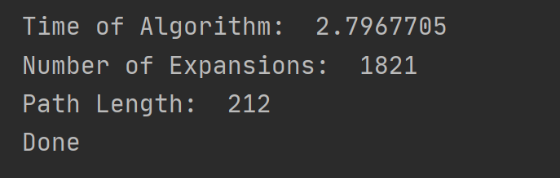
\includegraphics[width=.8\linewidth]{fastbackAstats.png}
  \label{fig:sfig2}
\end{subfigure}
\caption{Faster Backward A*}
\end{figure}
\setcounter{figure}{0}


\newpage

\section*{Part 4: Heuristics in Adaptive A*}
\subsubsection*{The project argues that “the Manhattan distances are consistent in grid worlds in which the agent can move only in the four main compass directions.” Prove that this is indeed the case.}
The Manhattan Distance is a heuristic that calculates the distance between two nodes limiting the movement to strictly vertical and horizontal movements. Since we limit the agents movement to only vertical and horizontal moves, it means that The Manhattan Distance will be a perfect estimation on a non blocked grid, or an underestimation on a blocked grid, making this heuristic consistent. If the agent was allowed to move diagonally, then this heuristic would be an overestimation because it would take less moves for the agent to get to the goal.



\subsubsection*{Furthermore, it is argued that “The h-values \texorpdfstring $h_{new}(n))$... are not only admissible but also consistent.” Prove that Adaptive A* leaves initially consistent h-values consistent even if action costs can increase.}

To prove this we will assume that $h(n)$ is the Manhattan Distance and \texorpdfstring $h_{new} = g(goal) - g(n)$\\
For a heuristic to be consistent, it will have to follow this inequality:
\[
  h(n) = c(n,a,n^{'}) + h(n^{'})  
\]
Now to prove that $h_{\text new} = c(n,a,n^{'}) + h_{\text new}(n^{'})$ We will have to substitute $h_{new} = g(goal) - g(n)$ into the above formula.
\[
    g(goal) - g(n) \leq c(n,a,n^{'}) +  g(goal) - g(n^{'})
\]
Simplify:
\[
    g(n) \geq g(n^{'}) + c(n,a,n^{'})
\]

Since $c(n,a,n^{'})$ is our action cost and can only be equal to one, our formula is consistent.
To prove that h(n) will continue to be consistent even while action cost increase we will substitute into the formula: 
\[
    h_{new}(n) \leq h_{new}(n^{'}) + c(n,a,n^{'}) \leq h_{new}(n^{'}) + c(n,a,n^{'})^{'}
\]
Proving that it is consistent even if the action costs can increase.



\setcounter{figure}{3}
\section*{Part 5: Heuristics in Adaptive A*}
\subsubsection*{Implement and compare Repeated Forward A* and Adaptive A*
with respect to their run-time. Explain your observations in detail, that is, explain what you observed and give a reason for
the observation. Both search algorithms should break ties among cells with the same f-value in favor of cells with larger
g-values and remaining ties in an identical way, for example randomly.
}
\clearpage
\setcounter{figure}{2}

\begin{figure}[h!]
  
  \centering
  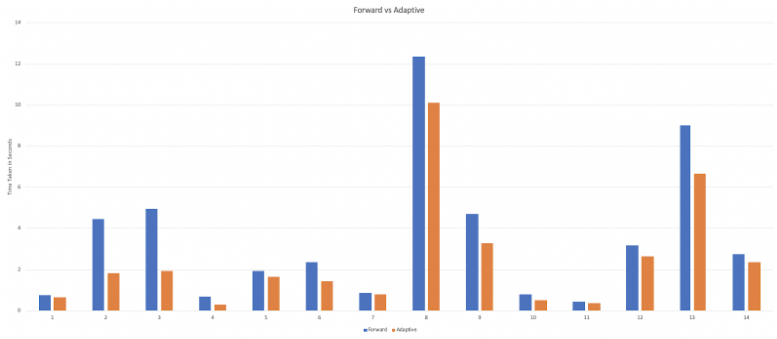
\includegraphics[width=0.8\textwidth]{graph3.png}
  \caption{Avg run-times: Forward A*: 3.51s, Adaptive A*: 2.46s}
\end{figure}

\setcounter{figure}{0}


After comparing Repeated Forward A* and Adaptive A*, we see that Adaptive A* runs much faster than Repeated Forward A* on an average aside from a few cases where the run-times are closer. This is because Adaptive A* results in a much lower number of expansions which changes the heuristic from the previous run of A*.
\newline



\begin{figure}[h!]
  
  \centering
  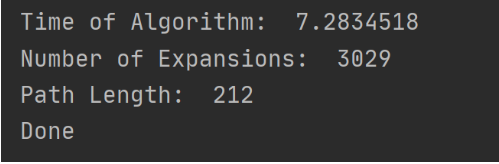
\includegraphics[width=0.5\textwidth]{repforwardstats.png}
  \caption{Repeated A*}
\end{figure}

\begin{figure}[h!]
  
  \centering
  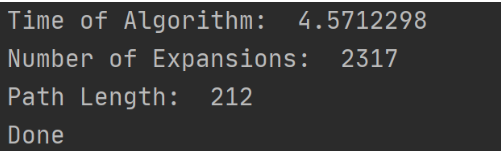
\includegraphics[width=0.5\textwidth]{adaptivestats.png}
  \caption{Adaptive A*}
\end{figure}


\section*{Part 6: Memory Issues}
\subsubsection*{Suggest additional ways to reduce the memory consumption of your implementations further.}
For us to reduce the amount of memory consumed we could change the way we implement our class Node. Currently it can hold the following attributes:  a nodes value (int), x-coordinate (int), y-coordinate (int), g-value (int), h-value (int), f-value (int), neighbors (list),  previous (node), adjust (bool). We can reduce these attributes by holding external maps of each of the values g, f, and h. We could calculate the neighbors during each loop instead of storing them as a list. We could also use a pointer for previous instead of sending the reference to the node.Instead of using a grid like structure we could have implemented the structure using just x and y values stored in a tuple or list.
\subsubsection*{Then,
calculate the amount of memory that they need to operate on grid-worlds of size 1001 × 1001 and the largest grid-world that
they can operate on within a memory limit of 4 MBytes.}
We use sys.getsizeof(cols[i][j]) to get the size of each cell, this came out to be 24 bytes.\\\\
\textbf{To get the size for a 1001x1001 grid: }
\[
	1001 * 1001 * 24 = 24.05 \text{MB}
\]
We are able to run a grid of size 408x408 when limited to 4MB.


%----------------------------------------------------------------------------------------
%	PROBLEM 1
%-------------------------------------------------------------------------------------------------------

\end{document}
